\section{An Analysis of Principles} \label{sec_converging_principles}

In this section, we will apply a systematic cross-referencing approach to each of the
principles of \gls{ca} with \gls{ns}. By cross-referencing these principles, we aim to
uncover the degree of convergence between \gls{ca} and \gls{ns} from a theoretical
perspective supported by examples from the artifacts. Along this explanation, the level
of convergence is denoted as follows:

\begin{table}[H]
    \begin{tabular}{ l l p{0.57\linewidth}} 
        
    Strong convergence & \fullConvergence & This indicates that the principles of \gls{ca} and \gls{ns}
    are highly converged. Both have a similar impact on the design and implementation of the
    artifact. \\
        
    Supports convergence & \npartialConvergence & The \gls{ca} principle supports
    implementing the \gls{ns} principle through specific design choices. However, applying
    the \gls{ca} principle does not inherently ensure adherence to the corresponding
    \gls{ns} principle. \\
        
    No or weak convergence & \noConvergence & The principles have no significant similarities
    in terms of their purpose, goals, or architectural supports \\
    \end{tabular}
\end{table}

\subsection{Single Responsibility Principle} \label{srp}

\evaluatePrincipleTable{\gls{srp}}{table_srp_alignment}{ \addEvalRow{\gls{soc} & \fullAlignment &
    The main goal of both \gls{srp} and \gls{soc} is to promote and encourage modularity,
    low coupling, and high cohesion. While the definition has some differences, the two
    principles can be regarded as practically interchangeable. Many examples in the
    Artifacts show a strong alignment between \gls{srp} and \gls{soc}. To name one, an
    Expander should be able to can perform multiple Tasks to complete the full
    instantiation of the Model. Each of those Tasks can be implemented separately from
    each other. Figure \ref{fig_handlers} illustrated some of the Tasks that are
    implemented in the Clean Architecture Expander Artifact. The Code Listing
    \ref{list_entityexpander} is an example of one implementation of such a Task
    \citecode{koks_expandentitieshandlerinteractor_2023}.}
    
    \addEvalRow{\gls{dvt} & \partialAlignment & Although using \gls{srp} does not
    implicitly guarantees \gls{dvt}, it does support \gls{dvt} by directing certain design
    choices. For example, both \gls{ca} and \gls{ns} assign specific \gls{dto} objects to
    support specific use cases (Interactors or Tasks) or to transfer (parts of) Data
    between architectural layers. \gls{ca} specifically assigned \glspl{dto} and
    guidelines on where and when to use them. These are also applied in the Artifact of
    this study as ResponseModels, RequestModels, and ViewModels
    \parencites{koks_requestmodels_2023,koks_viewmodels_2023}. The separation of data
    structures specific to Use Cases minimizes the impact of data structure changes by
    preferring stamp coupling over data coupling. However, \gls{srp} is not a guaranteed
    measure for \gls{dvt}.}
    
    \addEvalRow{\gls{avt} & \partialAlignment & While \gls{srp} emphasizes limiting the
    responsibility of each module, it does not explicitly require handling specific
    versions of use cases. Nevertheless, adhering to gls{srp} can still indirectly
    contribute to achieving \gls{avt}. One way to achieve this is by separating versions
    of Actions into separate contracts, objects, or methods, enabling Action Version
    transparency to some degree. Although not yet available in the Artifact, the Code
    Listing \ref{list_versioning} shows that API versioning is a common standard practice
    and fully supported by the open API specifcation and the .net core framework
    \parencites{github_aspnet-api-versioningprogramcs_2023, oas_versioning_2023}.
    Manifestations in the Artifact can be located in the Logger (Code Listing
    \ref{list_logging}), amongst others \parencite*{koks_logger_2023}.}
    
    \addEvalRow{\gls{sos} &\noAlignment & Following \gls{srp} might lead to separate modules
    that manage their state, indirectly contributing to \gls{sos}. However, the alignment
    is very weak, and no manifestations are found in the artifacts.}

}

\begin{figure}[H]
    \centering
    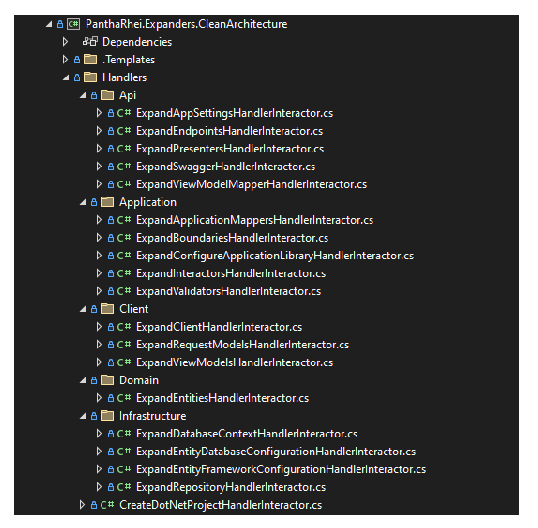
\includegraphics[width=0.6\textwidth]{figures/expander_handlers.pdf}
    \caption[handlers]{Each of the handlers handles an isolated part of the expanding process.}
    \label{fig_handlers}
\end{figure}
\subsection{Open/Closed Principle}

\evaluatePrincipleTable{\acrshort{ocp}}{table_ocp_convergence}{ 
    
\addEvalRow{\gls{soc} & \fullConvergence & The \gls{ocp} strongly converges with
    the \gls{soc} principle of \gls{ns}. \gls{ocp} states that software architectures
    should be open for extension but closed for modification. When applying \gls{ocp}
    correctly, the architecture supports new requirements built as an extension, affecting
    as few existing implementations as possible. Conversely, adhering to \gls{soc} does
    not guarantee adherence to \gls{ocp}, as \gls{soc} focuses on modularization and
    encapsulation rather than the extensibility of functionality. The same example with
    the Tasks provided in sub-section \ref{srp} is also an excellent manifestation of this
    principle.} 
    
\addEvalRow{\gls{dvt} & \noConvergence & The \gls{ocp} indirectly relates to the \gls{dvt}
principle. The convergence of both principles is weak, and no manifestations are found in
the artifacts.}
    
\addEvalRow{\gls{avt} & \fullConvergence & The \gls{ocp} strongly converges with the
    \gls{avt} principle of \gls{ns}, as both principles emphasize the importance of
    allowing changes or extensions to actions without affecting existing implementations.
    \gls{ocp} is also closely related to \gls{srp}. Besides \gls{srp}, \gls{ocp} has the
    most manifestations in the artifact, some of which are already mentioned in previous
    examples. } 
    
\addEvalRow{\gls{sos} & \noConvergence & The \gls{ocp} indirectly relates to the \gls{sos}
    principle. The convergence of both principles is weak, and no manifestations are found
    in the artifacts. } }
\subsection{Liskov Substitution Principle}

\evaluatePrincipleTable{\gls{lsp}}{table_lsp_alignment}{ 
    
\addEvalRow{\gls{soc} & \fullAlignment & \gls{lsp} states that objects of a derived class should be
able to replace objects of the base class without affecting the program negatively.
Replacing objects can only be achieved by separating them, aligning the principles
inherritly. A good example is the implementation of the
\citecode{koks_itemplateinteractor_2023} where the template engine Scriban
\parencite{github_scriban_2023} is used to generate code instantiations as a result of the
Expanding the Model \parencite{koks_scribantemplateinteractor_2023}. We could easily
replace the Scriban template engine for an other engine with only impacting the Dependency
Injection Register.}
    
\addEvalRow{\gls{dvt} & \noAlignment & The alignment between \gls{lsp} and \gls{dvt} is weak,
and no manifestations are found in the artifacts.}
    
\addEvalRow{\gls{avt} & \partialAlignment & The \gls{lsp} supports the \gls{avt} principle.
Both principles emphasize the importance of allowing the extensibility of the software
system. By adhering to \gls{lsp}, the architecture allows for class hierarchies that can
be easily extended to accommodate new (versions of) actions, which can contribute to
achieving \gls{avt}. However, adhering to \gls{lsp} alone may not guarantee full adherence
with \gls{avt}. Considder \citecode{koks_icreategateway_2023} in Code Listing
\ref{list_ICreateGatewayExamples}. The artifact contains multiple implementations of this
interface. Each implementation could be considered a different version applied to the
interface.} 
    
\addEvalRow{\gls{sos} & \noAlignment & The \gls{lsp} does not relate to the \gls{sos}
principle. The alignment of both principles is weak, and no manifestations are found in
the artifacts.} }

\subsection{Interface Segregation Principle}

\evaluatePrincipleTable{\gls{isp}}{table_isp_convergence}{ 
    
\addEvalRow{\gls{soc} & \fullConvergence & The \gls{isp} strongly converges with the
\gls{soc} principle, as both emphasize the importance of modularity and the separation of
concerns. \gls{isp} states that clients should not be forced to depend on implementation
they do not use, promoting the creation of smaller, focused interfaces. Listing
\ref{list_ispexample} shows that each \gls{crud} operation has its own interface
\parencite{koks_crudgateways_2023}.}
    
\addEvalRow{\gls{dvt} & \noConvergence & The \gls{isp} does not relate to the \gls{dvt}
principle. The convergence of both principles is weak, and no manifestations are found in
the artifacts.}
    
\addEvalRow{\gls{avt} & \npartialConvergence & The convergence between \gls{isp} and
\gls{avt} arises from the emphasis of \gls{isp} on creating targeted interfaces tailored
to specific needs. Smaller interfaces can enhance modularity and minimize unwanted side
effects when modifying Actions in the software system, positively impacting the
implementation of the \gls{avt}. For example, modifications in Actions are likely to have
a limited impact. However, adhering to \gls{isp} is not a guarantee for \gls{avt}.} 
    
\addEvalRow{\gls{sos} & \noConvergence & The \gls{isp} does not relate to the \gls{sos}
principle. The convergence of both principles is weak, and no manifestations are found in
the artifacts.} 

}
\subsubsection{The Dependency Inversion Principle} \label{subsubsec_dip} 
\textcolor{red}{
TODO: explain how dependency injection can benefit the implementation and align with
\ref{tab_convergence_dip}}

The \gls{dip} prescribes that high-level modules should not depend on low-level modules,
and that both should depend on abstractions. The principle emphasizes that the
architecture should be designed in such a way that the flow of control between the
different objects, layers and components are always from higher-level implementations
to lower-level details.

In other words, high-level implementations like business rules, should not be concerned
about low-level implementations, such as the way the data is stored or presented to the
end user. Additionally, both the high-level and low-level implementations should only
depend on abstractions or interfaces that define a contract for how they should interact
with each other \parencite[109]{robert_c_martin_clean_2018}.

This approach allows for great flexibility and a modular architecture. Modifications in
the low-level implementations will not affect the high-level implementations as long as
they still adhere to the contract defined by the abstractions and interfaces.
Similarly, changes to the high-level modules will not affect the low-level modules as long
as they still fulfill the contract. This reduces coupling and ensures the evolvability
system over time, as changes can be made to specific modules without affecting the rest of
the system.

Manifestations in the artifacts are ample. One of which is the consistent use of the
Dependency Injection pattern. In order to prevent the risks of displacing and dispersing
dependencies all over the system \parencite[214]{mannaert_normalized_2016} we are using
dependency containers. Each module is maintaining its own dependencies, which are
bootstrapped at application startup (see Listing \ref{list_dip})
\parencite{koks_generator_2023}.

\lstinputlisting[
    caption={Bootstrapping the dependencies of each component/layer of the
    generator artifact.},
    label={list_dip}]
    {Snippets/Dip.cs}

A more abstract example is the separation of required modules into separate component
libraries. This applies to both the generated and generator artifact (see Figure
\ref{fig_solutions}). The actual compliance to the \gls{dip} is how the flow of control
between the components is organized. This is accurately depicted in Figure
\ref{fig_modulair_components} \nameref{fig_modulair_components}.

\begin{figure}[H]
    \centering
    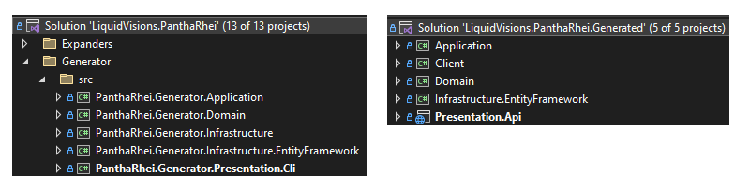
\includegraphics[width=1\textwidth]{figures/solutions.pdf}
    \caption[Separation of component libraries]{Separation of component libraries.}
    \label{fig_solutions}
\end{figure}
\subsection{The Principles Convergence Overview}

In this section, we will apply a systematic cross-referencing approach to each of the
principles of \gls{ca} with \gls{ns}. By cross-referencing these principles, we aim to
uncover the degree of convergence between \gls{ca} and \gls{ns} from a theoretical
perspective, supported by examples from the artifacts. Along with this explanation, the
level of convergence is denoted as follows:

\begin{table}[H]
\renewcommand{\arraystretch}{1.5}
\centering
\begin{tabular}{r|llll}

    \textbf{\acrlong{ca}   } \textbf{   \rotatebox[origin=l]{90}{\acrlong{ns}}} & 
    \rotatebox[origin=l]{90}{\acrlong{soc}} & \rotatebox[origin=l]{90}{\acrlong{dvt}} &
    \rotatebox[origin=l]{90}{\acrlong{avt}} & \rotatebox[origin=l]{90}{\acrlong{sos}} \\
\midrule


\acrlong{srp} & \fullConvergence & \npartialConvergence & \npartialConvergence & \noConvergence \\
\acrlong{ocp} & \fullConvergence & \noConvergence & \fullConvergence & \noConvergence \\
\acrlong{lsp} & \fullConvergence & \noConvergence & \npartialConvergence & \noConvergence \\
\acrlong{isp} & \fullConvergence & \noConvergence & \npartialConvergence & \noConvergence \\
\acrlong{dip} & \fullConvergence & \noConvergence & \npartialConvergence & \noConvergence \\
\bottomrule
\end{tabular}
\caption{An overview of the convergence of all \gls{ca} and \gls{ns} principles}
\label{tab_convergence_principles_summarized}
\end{table}


